\section{The architecture}

%The difficulty of person re-identification problem lies in several factors of person appearance variation, including lighting changes, different poses, different view points. Many challenges of person re-identification are shared with the fine-grained recognition task: one person can look very differently when captured by different cameras, and different persons can look similar if they wear similar clothes and can only be distinguishable based on a small outfit element.  Moreover, person re-identification and fine-grained classification have already been approached with related methods \citep{ma2012local, lin2015bilinear}. 
Our solution combines the state-of-the-art method for person re-identification (Deep Metric Learning  \citep{yi2014deep}, described in details in \sect{intro_architectures}) and the state-of-the-art fine-grained recognition method (bilinear CNN \citep{lin2015bilinear}). Modifying the bilinear CNNs by performing multi-region pooling boosts the performance of this combination significantly. Below, we introduce the notations and discuss the components of the system in detail.


% The baseline architecture, called Deep Metric Learning (DML), is described in details in \sect{intro_architectures}.
% We now give an in-depth review of both components, and then discuss how our architecture combines them. Finally, we motivate and discuss a further improvement over the straightforward combination that helps us to boost the re-identification performance.

%\indent\textbf{Convolutional architecture.} 

%We use the Deep Metric Learning (DML) architecture proposed by \citep{yi2014deep} as baseline, it is described in \sect{intro_architectures}.

%The CNN proposed by \citep{yi2014deep} incorporates ``siamese'' neural net, initially introduced for signature verification \citep{bromley1993signature} and later for face recognition in \citep{chopra2005learning}. The siamese architecture consists of two similar sub-networks for separate processing of two input images. 
%The network incorporates independent streams, in which three overlapping parts of person images are processed separately (top, middle and bottom parts), and produces  500-dimensional descriptor as an output.
%These sub-networks are responsible for calculating descriptors for a pair of images which are then connected via distance function.  Each of the two ``siamese'' sub-networks includes three independent streams, in which three overlapping parts of person images are processed separately, namely, the top part (head, upper torso), the middle part (torso), and the lower part (legs, lower torso). This is done in order to take into account different statistics of textures, shapes, and pose changing in different parts of the image, while still utilizing convolutional layers with spatially-invariant kernels. 

%Each of the three streams incorporates two convolutional layers of size $7\times7$ and $5\times5$, followed by the rectified linear (ReLU) non-linearity and max pooling with the kernel size of two pixels and the stride of two pixels.  %Each of the two sub-networks produces 500-dimensional descriptor vector as an output, and for each training pair of images the cosine similarity of these descriptors is calculated. At training time, the similarity value with the pair label (+1 for the same identity, -1 - for different identities) is then fed into the loss function.

%As in \citep{yi2014deep}, we consider the \textit{view-invariant} variant with the same weights shared for all views in the dataset. This case is more general as the trained networks can be used for new out-of-sample cameras, unlike the view-specific case that lacks weights sharing (which makes networks to capture view-specific appearance peculiarities).

 
% Unlike other approaches incorporating CNNs (\citep{li2014deepreid}, \citep{ahmed2015improved} and \citep{chen2015deep}), CNN uses a simple cosine similarity (equivalent to Euclidean distance between normalized descriptors) for the obtained image descriptors. Thus, photometric and geometric transforms specific for a pair of images are not modeled or inferred. On the other hand, as discussed above, descriptors produced with CNN are suitable for large-scale systems that need to use simple metrics.

\begin{figure*}
\begin{center}
    

\begin{tabular}{cc}
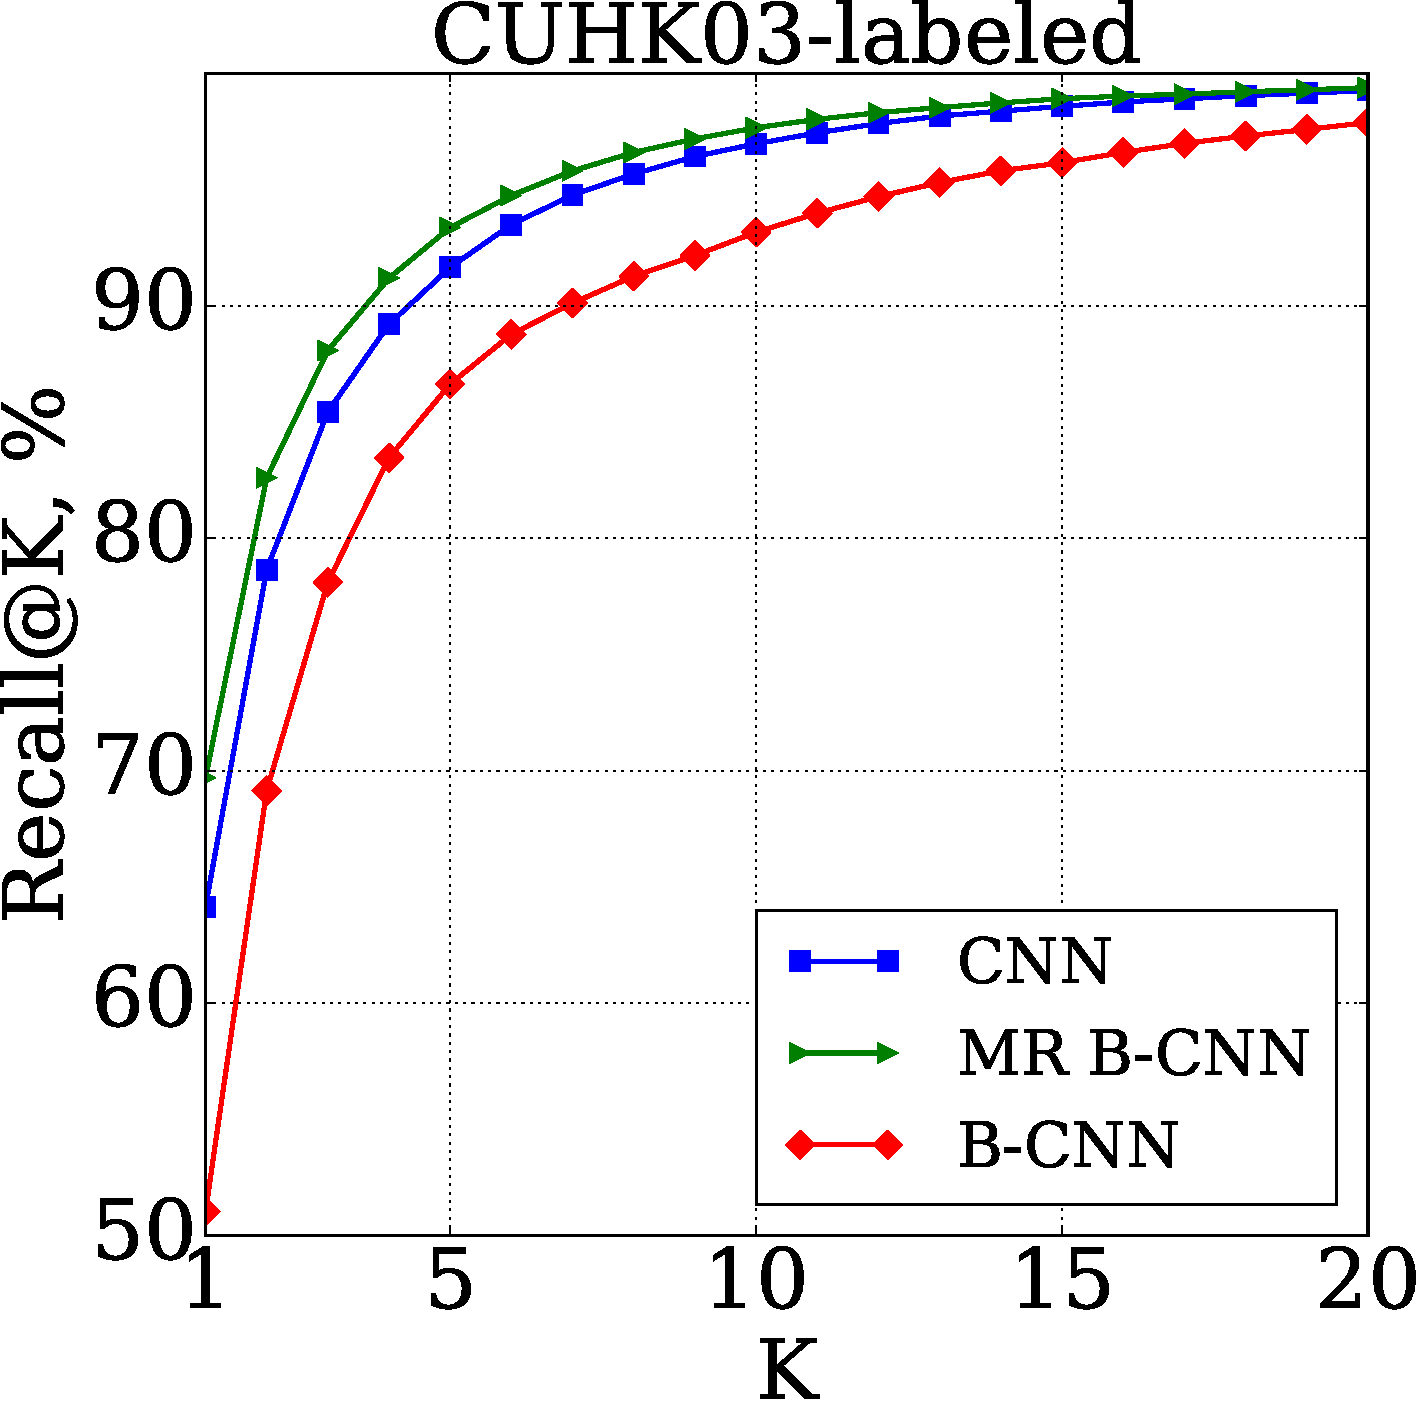
\includegraphics[width=0.6\textwidth]{\bilinearroot/figures/plots/cuhk03_labeled_different_arch_hist.pdf}\\
(a) \\
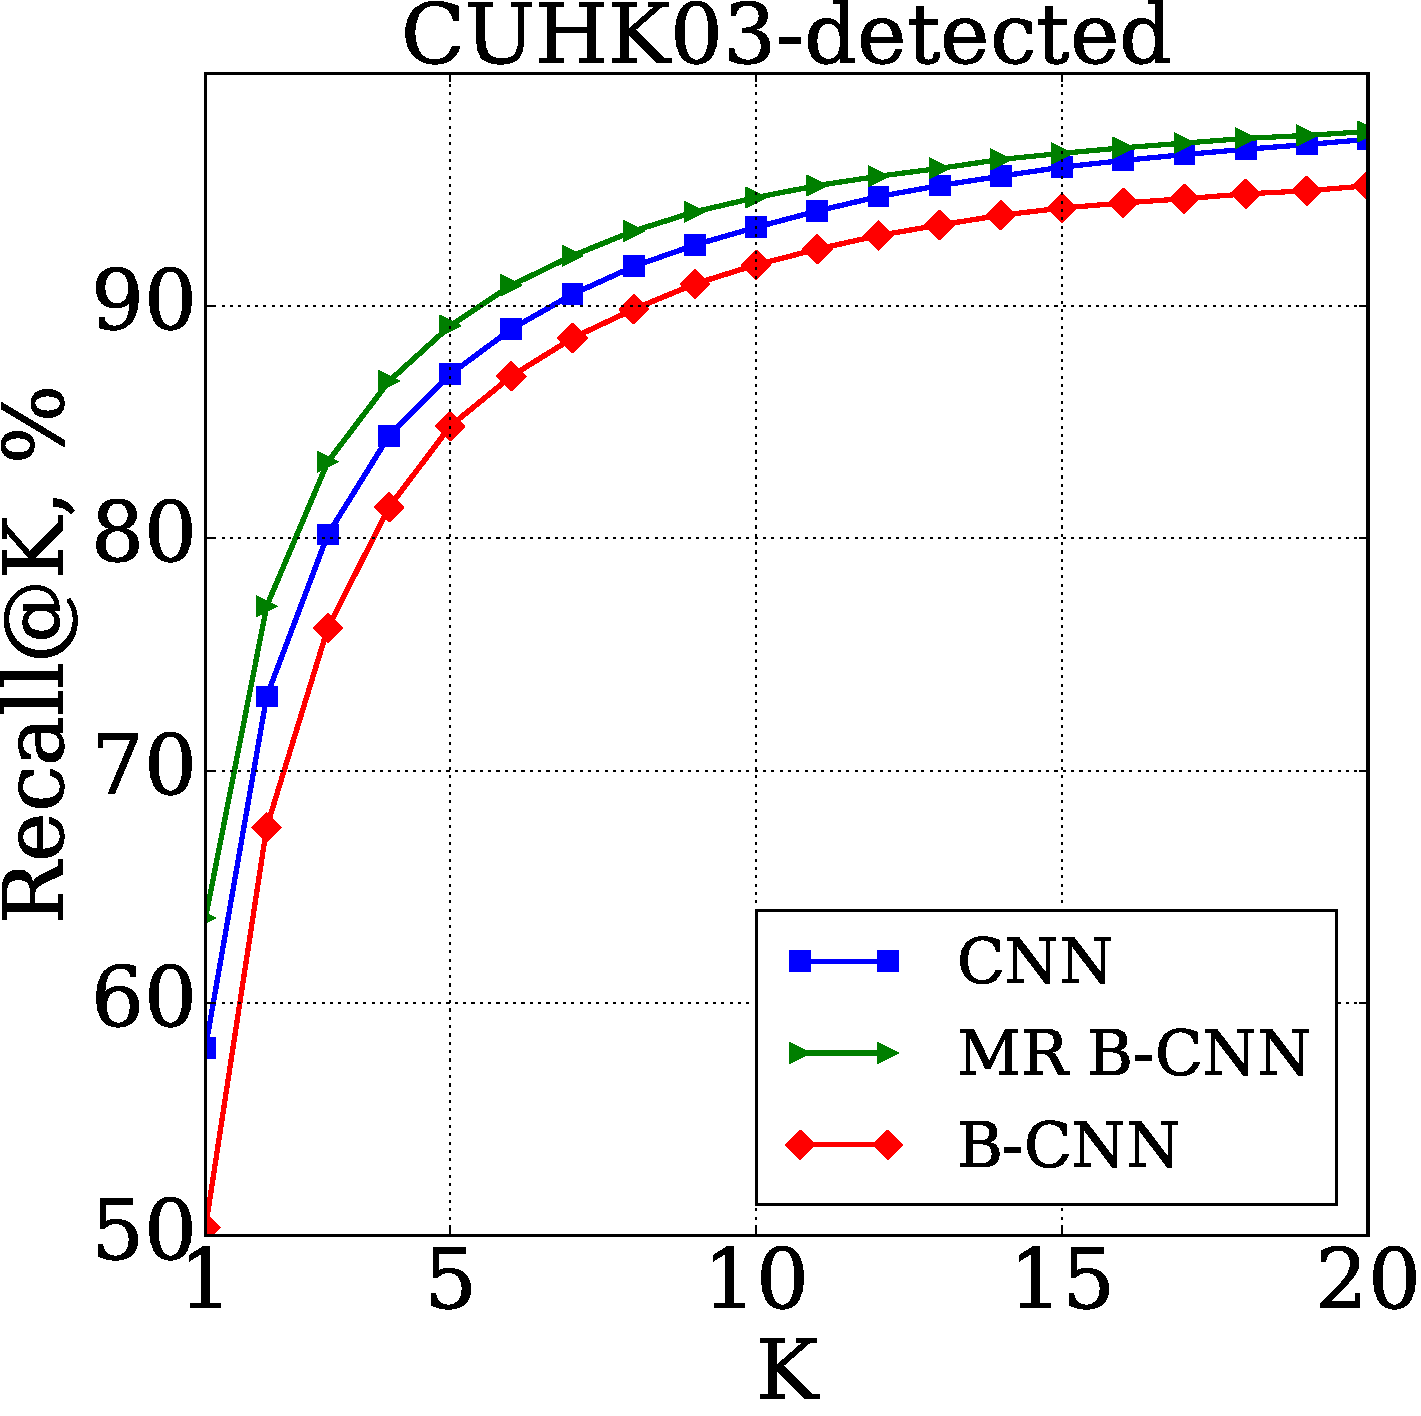
\includegraphics[width=0.6\textwidth]{\bilinearroot/figures/plots/cuhk03_detected_different_arch_hist.pdf}\\
(b) 

\end{tabular}
\caption{Recall@K results for the (a) CUHK03-labeled, (b) CUHK03-detected. MR B-CNN uniformly outperforms other architectures.}
\label{fig:recall}
\end{center}
\end{figure*}


\begin{figure*}
\begin{center}
    

\begin{tabular}{c}
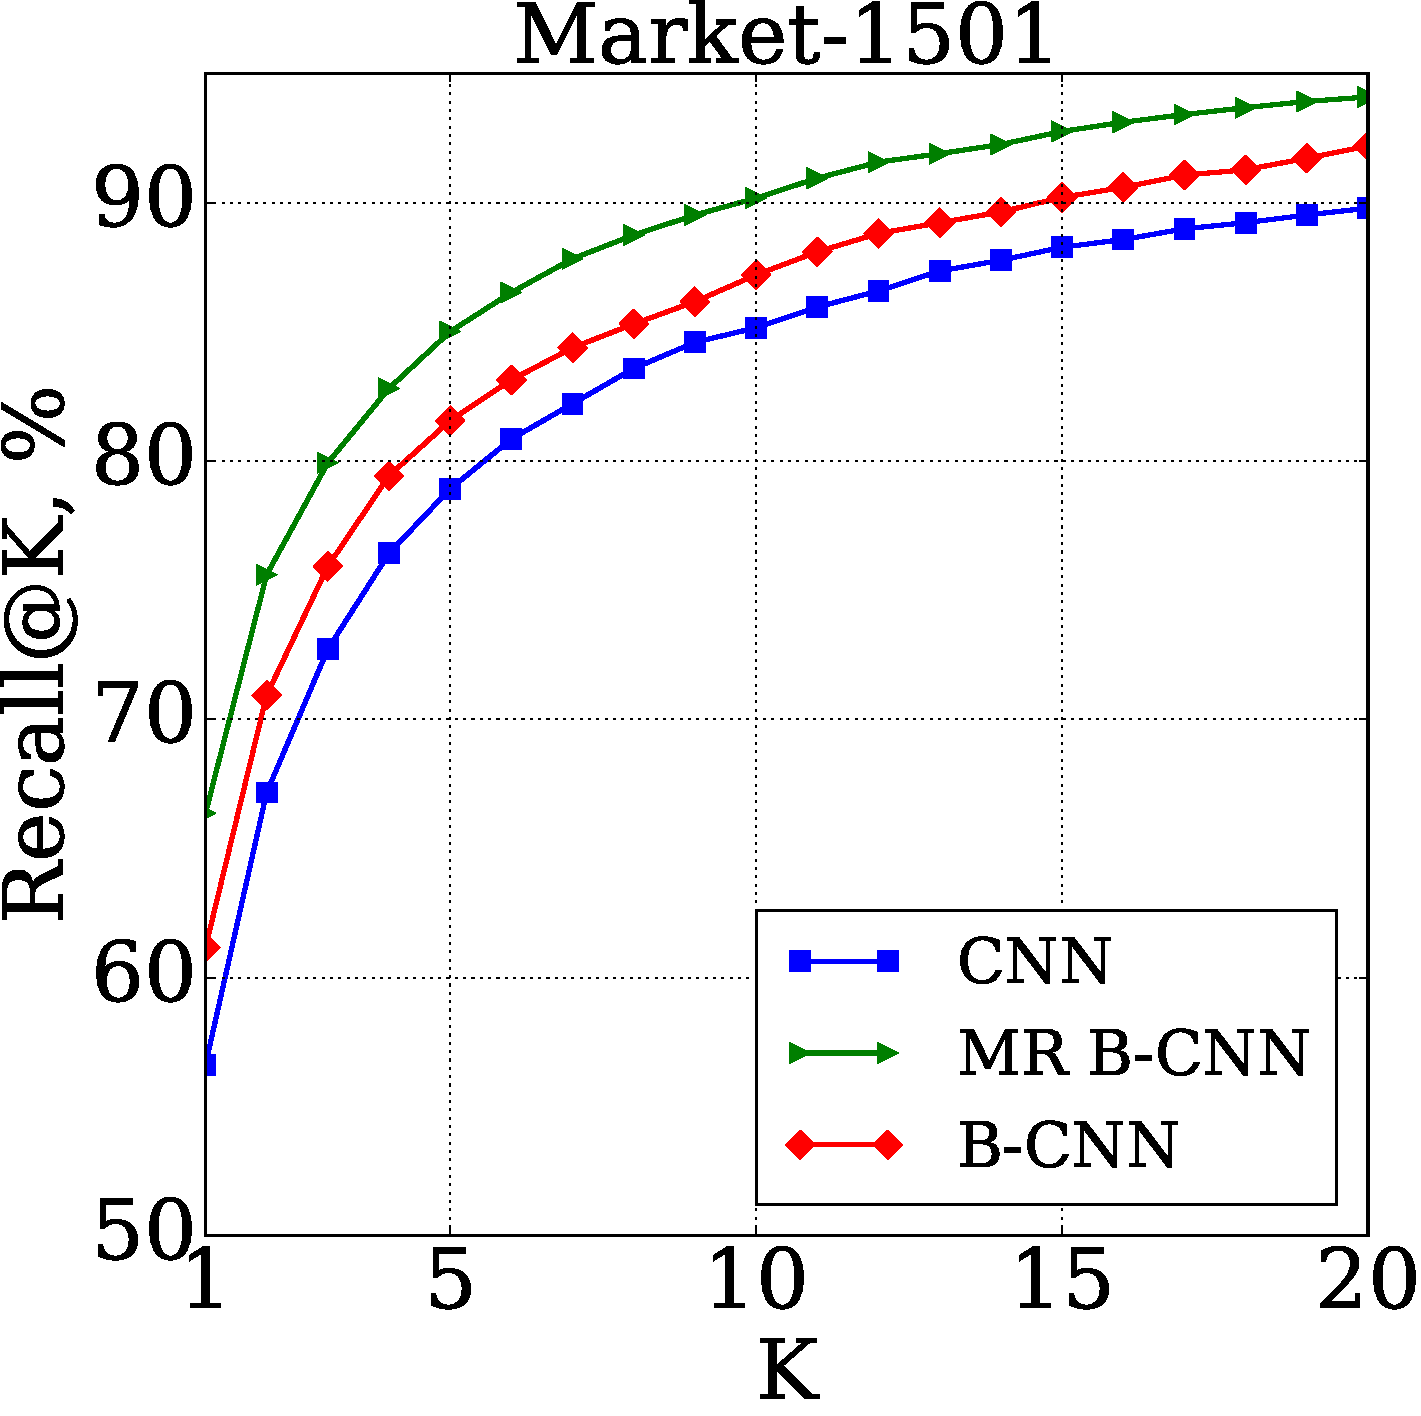
\includegraphics[width=0.6\textwidth]{\bilinearroot/figures/plots/market_different_arch_hist.pdf}\\
(a) \\
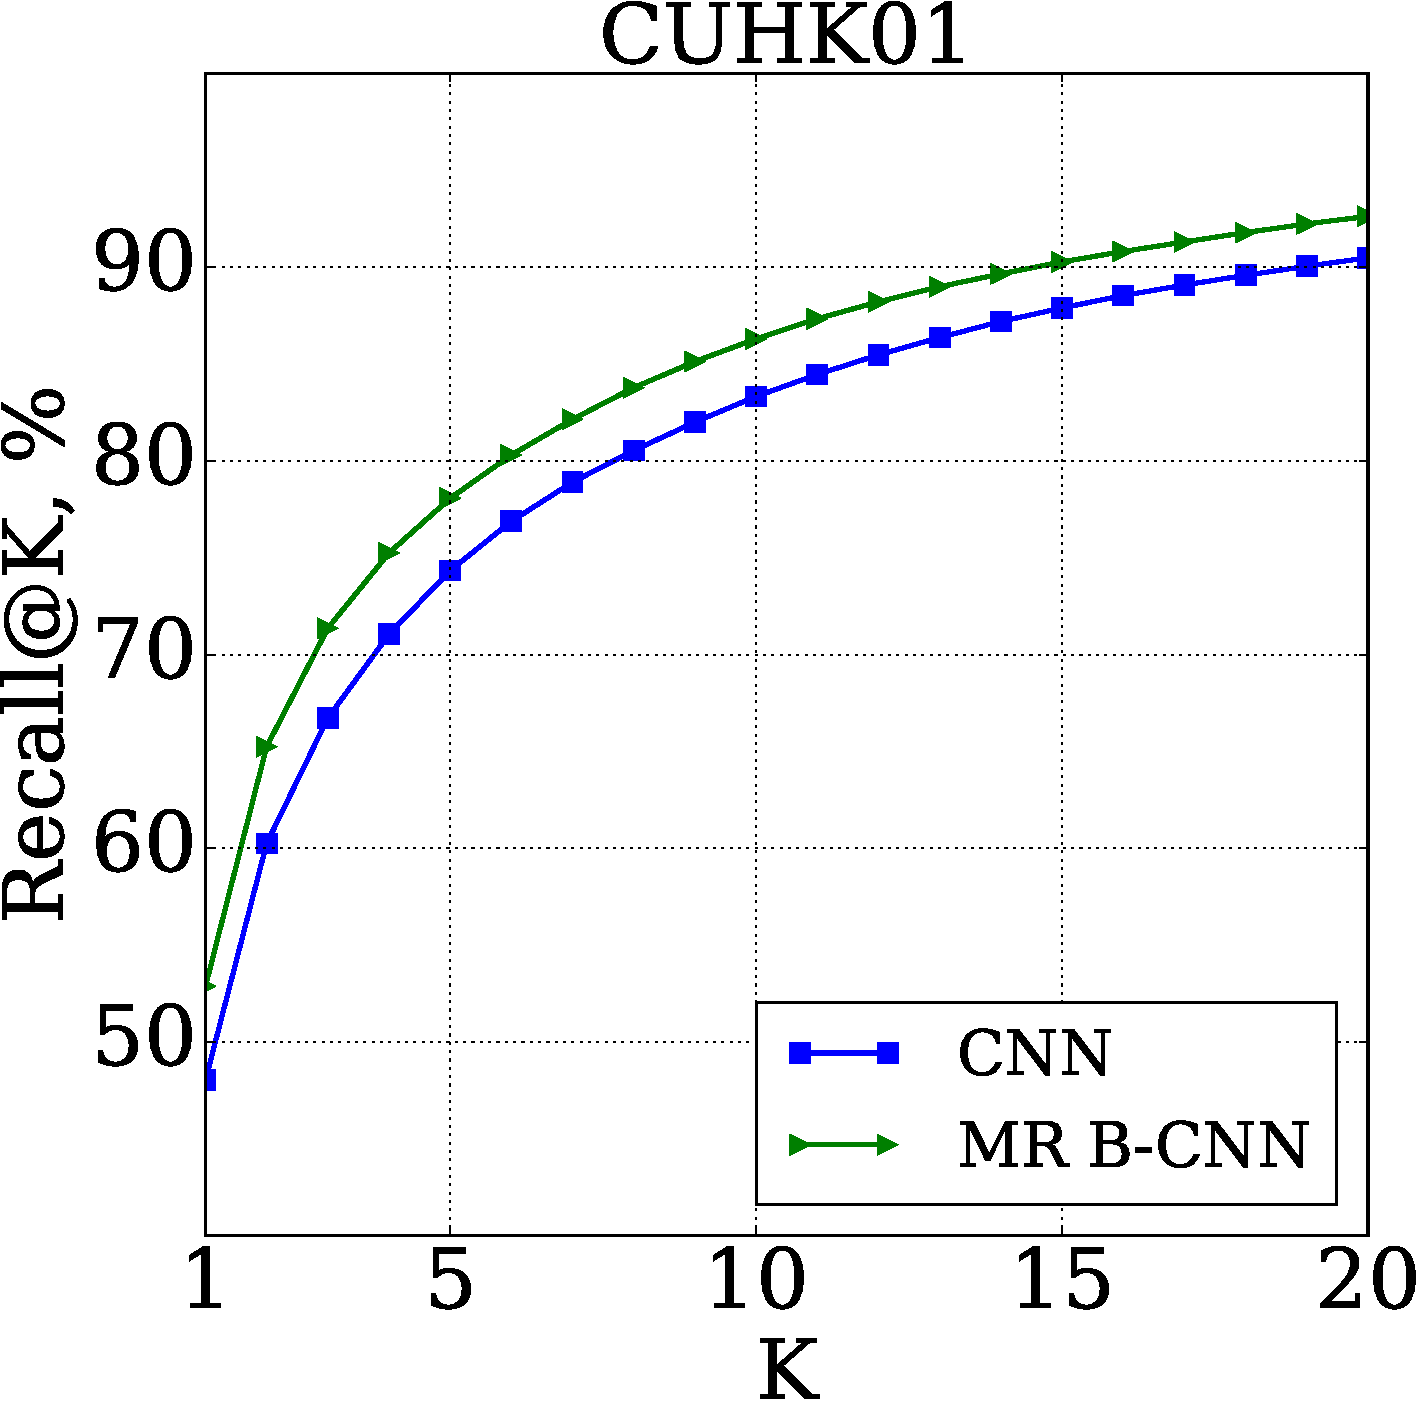
\includegraphics[width=0.6\textwidth]{\bilinearroot/figures/plots/cuhk01_different_arch_hist.pdf}\\
(b) \\
\end{tabular}
\caption{Recall@K results for the (a) Market-1501 (b) CUHK01, datasets. MR B-CNN uniformly outperforms other architectures.}
\label{fig:recall}
\end{center}
\end{figure*}

\indent\textbf{Multi-region Bilinear Model.}\\
Bilinear CNNs are motivated by the specialized pooling operation that aggregates the correlations across maps coming from different feature extractors. The aggregation however discards all spatial information that remains in the network prior to the application of the operation. This is justified when the images lack even loose alignment (as e.g.\ in the case of some fine-grained classification datasets), however is sub-optimal in our case, where relatively tight bounding boxes are either manually selected or obtained using a good person detector.  Thus some loose geometric alignment between images is always present. Therefore we modify bilinear layer and replace it with the  \textit{multi-region bilinear layer}, which allows us to retain some of the geometric information. Our modification is, of course, similar to many other approaches in computer vision, notably to the classical spatial pyramids of \citep{Lazebnik06}.
In more detail, similarly to \citep{lin2015bilinear}, we introduce the bilinear model for image similarity as follows: 
\\ $\mathcal{B} = ({f_{A}^{}}, {f_{B}^{}}, \mathcal{P}, \mathcal{S})  $, where ${f_{A}^{}}$ and ${f_{B}^{}}$ are feature extractor functions (implemented as CNNs), $\mathcal{P}$ is the pooling function, $\mathcal{S}$ is the similarity function. The feature function takes an image ${\mathcal{I}}$ at location $\mathcal{L}$ and outputs the feature of determined dimension $\mathcal{D}$ (unlike \citep{lin2015bilinear}, we use vector notation for features for simplicity): $f : \mathcal{I} \times \mathcal{L} \rightarrow \mathcal{R}_{}^{1 \times \mathcal{D}}$. In this work, two convolutional CNNs (without fully-connected layers) serve as the two feature extractors $f_{A}^{}$ and $f_{B}^{}$. For each of the two images in the pair at each spatial location, the outputs of two feature extractors $f_{A}^{}$ and $f_{B}^{}$ 
are combined using the bilinear operation \citep{lin2015bilinear}: 
\begin{equation}
 \label{eq:bilinear}
\text{bilinear}(l, im, {f_{A}^{}}, {f_{B}^{}}) = {{f_{A}^{}}(l, im)_{}^{T}{f_{B}^{}}(l, im)},
\end{equation}
where $l \in \mathcal{L}, im \in \mathcal{I}$.
Using the operation \eq{bilinear}, we compute the bilinear feature vector for each spatial location $l$ of the image $im$. If the feature extractors $f_{A}^{}$ and the $f_{B}^{}$ output local feature vectors of size $M$ and $N$ correspondingly, their bilinear combination will have size $M \times N$ or $MN \times 1$, if reshaped to the column vector. 

We then suggest to aggregate the obtained bilinear features by pooling across locations that belong to a predefined set of image regions:  ${r_{1}},  ..., {r_{R}}$, where $R$ is number of chosen regions.
After such pooling, we get the pooled feature vector for each image region $i$ (as opposed to the feature vector that is obtained in \citep{lin2015bilinear} for the whole image):
\begin{equation} \label{eq:bilinear_pooling}
\phi_{r_{i}}(im) = \phi(im_{r_{i}}) = \sum_{l \in r_{i}} \text{bilinear}(l, im, {f_{A}^{}}, {f_{B}^{}})
\end{equation}

Finally, in order to get a descriptor for image $im$, we combine all region descriptors into a matrix of size $R \times MN$:
\begin{equation} \label{eq:desc}
\phi(im) = [{\phi_{r_{1}}(im)}_{}^{T}; {\phi_{r_{2}}(im)}_{}^{T}; ... ; {\phi_{r_{R}}(im)}_{}^{T}]. 
\end{equation}




%This matrix can be turned into a vector descriptor by reshaping. Alternatively, some transforms can be applied beforehands. Formally, such additional transforms can be incorporated into the similarity function $\mathcal{S}$. For example, fully connected layer can perform additional feature transformation within our architecture. Note, that for some types of transforms (for example, for convolution) the spatial order of pooling regions should be preserved.

To pick the set of regions, in our experiments, we simply used the grid of equally-sized non-overlapping patches (note that the receptive fields of the units from different regions are still overlapping rather strongly). The scheme of Multi-region Bilinear CNN architecture is shown in figure~\ref{fig:architecture}a. \\
We incorporate the multi-region bilinear operation (\ref{eq:desc}) into the convolutional architecture in the following way: instead of using one sub-network for each image part, we use two feature extractors with the same convolutional architecture described above. The outputs are combined by the multi-region bilinear operation (\ref{eq:desc}) after the second convolution. Three bilinear outputs for each of the image parts are then concatenated and turned into a 500-dimensional image descriptor by an extra fully connected layer.  The overall scheme of Multi-region Bilinear CNN net for each of the two siamese sub-networks used is this work is shown in figure \ref{fig:architecture}b.


% \indent\textbf{Learning the model.}\\
% %We now discuss the combination of Deep Metric Learning (CNN) and Bilinear CNN (Bilinear-CNN) architectures.
% As in \citep{yi2014deep}, we use deep embedding learning \citep{chopra2005learning}, where multiple pedestrian images are fed into the identical neural networks and then the loss attempts to pool descriptors corresponding to the same people (\textit{positive or matching pairs}) closer and the descriptors corresponding to different people (\textit{negative or non-matching pairs}) apart. To learn the embeddings, we use the Histogram loss introduced in \chapt{hist}. %Specifically, this loss generates all possible positive and negative pairs within each mini-batch and calculates cosine similarities for them, after which the histograms for the two distributions corresponding to the cosine similarities between matching and non-matching pairs are estimated. The final loss value is then calculated using the two histograms as the probability of the arbitrary positive and negative similarities to be in wrong order (more details about this embedding loss can be found in \citep{UstinovaNIPS16}).
%in the following way. 
% \begin{equation} \label{eq:hist}
%     \hp_r = \frac{1}{|\Sp|}\sum_{(i,j)\,:\,m_{ij}=+1} \delta_{i,j,r}\, 
% \end{equation}
% where $(i,j)$ are all the positive or  pairs in the batch. And  $\delta_{i,j,r}$ are the weights of assignment the similarity to adjacent nodes of the regular grid with еру cell of size $\Delta$:
% \begin{equation} \label{eq:histweight}
% \delta_{i,j,r} = \begin{cases} 
%     (s_{ij}-t_{r-1})/\Delta,\; &\text{if $s_{ij} \in [t_{r-1};t_r]$},\\
%     (t_{r+1}-s_{ij})/\Delta,\; &\text{if $s_{ij} \in [t_r;t_{r+1}]$},\\
%     0,\; &\text{otherwise}\,.
%     \end{cases}
% \end{equation}
% The final loss value is then calculated using the two histograms as the probability of the arbitrary positive and negative similarities to be in wrong order: 
% \begin{equation} \label{eq:loss}
% L = \sum_{r=1}^R \left( \hm_r \sum_{q=1}^r \hp_q  \right)\,,
% \end{equation}
% where $R$ is the number of nodes used for histogram estimation, $\hp$ and $\hm$ are the aggregated histograms for the matching and the non-matching pairs similarities.


%Similar to \citep{yi2014deep}, we use cosine similarity function and the Binomial Deviance loss function: 
%\begin{equation}
%\label{eq:bindev}
% J_{dev} = \sum_{i,j \in I} w_{i,j} \ln (\exp^{-\alpha (s_{i,j}-\beta) m_{i,j}} +1 ), 
% \end{equation}

% where $I$ is the set of training image indices, and $s_{i,j}$ is the similarity measure between $i$th and $j$th images (i.e.\ $s_{i,j} = cosine(x_{i}, x_{j}$).

% Furthermore,  $m_{i,j}$ and $w_{i, j}$ are the learning supervision and scaling factors respectively:
% \\$ m_{i, j} = \left\{
% 	\begin{array}{l l}
% 		1,  ${if $(i,j)$ is a positive pair}$ &\\
% 	   -1,  ${if $(i,j)$ is a negative pair}$ &
% 	\end{array}
% 	\right.$ $w_{i, j}= \left\{
% 	\begin{array}{l l}
% 		\frac {1}{n_1},  ${if $(i,j)$ is a positive pair}$ &\\
% 		\frac {1}{n_2},  ${if $(i,j)$ is a negative pair}$ &
% 	\end{array}
% 	\right.$,
% 	where $n_1$ and $n_2$ are the number of positive and begative pairs in the training set (or training batch) correspondingly, $\alpha$ and $\beta$ are hyper-parameters. 




%Following the original architecture \citep{yi2014deep}, we use the two convolution layers with 64 output feature maps (filter size of the first one is 7$\times$7, and of the second one is 5$\times$5), followed by the rectified linear (ReLU) non-linearity and max pooling with the kernel size of two pixels and the stride of two pixels. 
%Also following \citep{yi2014deep}, we use separate sub-networks for the three parts of pedestrian images (head and upper torso, torso, legs and lower torso) to take into account different semantic nature of the  three parts. As in \citep{yi2014deep}, we have the weights of the first convolution layers  shared for the three sub-networks.

